\chapter{Fundamentals}
\section{Self-Sustained Oscillation}
Oscillation requires the loop gain magnitude to approach unity while the accumulated phase equals \((2k+1)\pi\) at the oscillation frequency. Because linear systems with unity loop gain drift, a nonlinear amplitude regulation mechanism is always present to stabilize the oscillation amplitude.

\section{Barkhausen Condition}
In small-signal sense, the Barkhausen condition states:
\[
|A(j\omega_0)\,\beta(j\omega_0)| = 1
\]
\[
\angle A\beta = (2k+1)\pi
\]
This is necessary for sustained oscillation but not sufficient for startup. For reliable startup, the magnitude condition should exceed unity at cold start:
\[
|A(j\omega_0)\,\beta(j\omega_0)| > 1
\]
so that noise or initial perturbations are amplified until nonlinear compression brings the loop to the steady-state limit cycle.

\section{Open-Loop and Closed-Loop View}
Consider a linear time-invariant forward path \(A(s)\) and feedback path \(\beta(s)\). The closed-loop characteristic equation is
\[
1 + A(s)\,\beta(s) = 0
\]
Oscillation arises when roots cross the imaginary axis at
\[
s = \pm j\omega_0
\]
In practice, the loop is slightly over-unity at startup (roots in the right-half plane), and settles to marginal stability by nonlinear amplitude compression at steady state.

\subsection*{Start-Up Gain Margin}
A practical design target is a start-up gain margin of
\[
M_{su} = |A(j\omega_0)\,\beta(j\omega_0)|
\]
with \(M_{su} \approx 2\) to 3, providing robustness to process, voltage, and temperature (PVT) variations while avoiding excessive distortion during amplitude build-up.

\section{LC Resonance and Quality Factor}
For an ideal LC tank, the natural frequency is
\[
f_0 = \frac{1}{2\pi\sqrt{LC}}
\]
Losses (e.g., series resistance of the inductor, dielectric loss of the capacitor) are captured by the quality factor, given by the series and parallel forms
\[
Q = \frac{\omega_0 L}{R_s}
\]
\[
Q = \frac{1}{\omega_0 R_p C}
\]
Higher \(Q\) implies lower damping, sharper resonance, and typically lower phase noise for LC oscillators.

\section{Negative Resistance View}
Practical LC VCOs implement an effective negative resistance \(-R_n\) that cancels tank loss \(R_p\). The small-signal start-up condition is
\[
|R_n| > R_p
\]
In steady state, device nonlinearity reduces \(|R_n|\) until \(|R_n| = R_p\), clamping the amplitude.

\section{Delay-Based Oscillation}
Ring oscillators exploit propagation delay around an inverting loop. If the total delay is \(N t_p\) for \(N\) identical stages, the oscillation frequency is approximately
\[
f \approx \frac{1}{2 N t_p}
\]
The tuning mechanism modifies \(t_p\) via bias current/voltage or load capacitance.

\section{Phase Noise Preliminaries}
Phase noise is the random fluctuation of the oscillator phase around the ideal uniform rotation. In the frequency domain, it appears as skirts around the carrier in the power spectral density (PSD). As a rule of thumb, LC oscillators achieve better phase noise than ring oscillators due to energy storage in high-\(Q\) tanks.

\subsection*{Numerical RMS Jitter Example}
Suppose the PN mask is $\{-80,-100,-120\}$ dBc/Hz at offsets $\{10\,\text{k}, 100\,\text{k}, 1\,\text{M}\}$ and $f_0=100\,\text{MHz}$. Converting to linear power and integrating by trapezoids over three bands yields an approximate integrated PN of $\sim 1.6\times10^{-9}$. Then
\[
 \sigma_t \approx \frac{1}{2\pi f_0}\,\sqrt{2\cdot 1.6\times10^{-9}} \approx 0.9\,\text{ps}_{\text{RMS}}
\]
This example is illustrative; actual values require the full mask and corner contributions \cite{hajimiri1998,demir2000}.

\section{Derivation Sketch of Barkhausen at Stability Boundary}
From the closed-loop characteristic equation
\[
1 + A(j\omega)\,\beta(j\omega) = 0
\]
the stability boundary occurs when poles lie on the imaginary axis. This implies
\[
|A(j\omega_0)\,\beta(j\omega_0)| = 1,\quad \angle A\beta = (2k+1)\pi
\]
Therefore Barkhausen represents the necessary condition for marginal stability of the oscillatory solution. Nonlinearities then enforce amplitude regulation to keep the loop on this boundary.

\section{Numerical Example: Ring VCO and \(K_{VCO}\)}
Assume a 3-stage ring with \(C_L = \SI{20}{\femto\farad}\), swing \(V_{swing} = \SI{0.6}{\volt}\), and bias current control \(I_{ctrl} \in [\SI{50}{\micro\ampere}, \SI{150}{\micro\ampere}]\). With \(t_p \approx C_L V_{swing}/I_{ctrl}\):
\[
t_p(I_{ctrl}) = \frac{20\times 10^{-15}\,\cdot\,0.6}{I_{ctrl}} = \frac{12\times 10^{-15}}{I_{ctrl}}\,\text{s}
\]
Hence the frequency is
\[
f(I_{ctrl}) \approx \frac{1}{2\,N\,t_p} = \frac{I_{ctrl}}{2\,N\,12\times 10^{-15}}\,\text{Hz}
\]
For \(N=3\):
\[
f(I_{ctrl}) \approx \frac{I_{ctrl}}{72\times 10^{-15}} = 13.9\times 10^{12}\cdot I_{ctrl}\,\text{(Hz/A)}
\]
Thus \(I_{ctrl}=\SI{50}{\micro\ampere}\Rightarrow f\approx \SI{695}{\mega\hertz}\), and \(I_{ctrl}=\SI{150}{\micro\ampere}\Rightarrow f\approx \SI{2.08}{\giga\hertz}\). If \(I_{ctrl} = g_m (V_{ctrl}-V_T)\), then \(K_{VCO} = (\partial f/\partial I_{ctrl})\,g_m\) provides a direct mapping to voltage tuning.

\section{Envelope Illustration}
\begin{figure}[H]
  \centering
  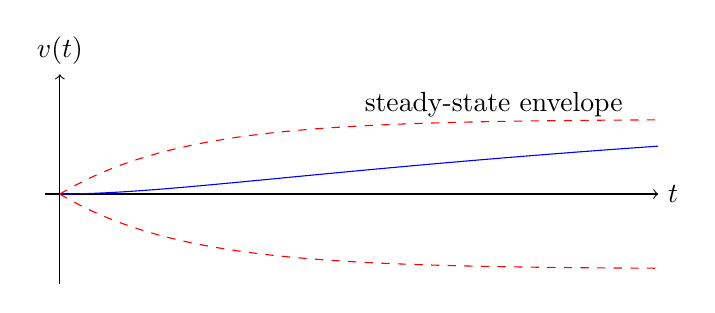
\begin{tikzpicture}[scale=0.95]
    \draw[->] (-0.2,0) -- (8,0) node[right] {$t$};
    \draw[->] (0,-1.2) -- (0,1.6) node[above] {$v(t)$};
    \draw[domain=0:8,samples=200,smooth,variable=\x,blue] plot (\x,{(1-exp(-0.6*\x))*sin(2*3.1416*0.8*\x)});
    \draw[red,dashed,domain=0:8,samples=100,smooth,variable=\x] plot (\x,{1-exp(-0.6*\x)});
    \draw[red,dashed,domain=0:8,samples=100,smooth,variable=\x] plot (\x,{-1+exp(-0.6*\x)});
    \node at (5.8,1.2) {steady-state envelope};
  \end{tikzpicture}
  \caption{Startup and steady-state envelope illustration}
\end{figure}

\section{Nonlinear Amplitude Regulation}
A simple envelope model writes the tank amplitude \(V(t)\) as
\[
\frac{dV}{dt} = (g(V) - \alpha)\,V
\]
where \(\alpha\) models loss and \(g(V)\) is the amplitude-dependent negative conductance. Near startup, \(g(0) > \alpha\) so \(V\) grows; at steady state, \(g(V_{ss}) = \alpha\), yielding a stable limit cycle. Polynomial or hyperbolic tangent models for \(g(V)\) capture device compression.

\section{Energy Perspective}
Let the tank energy be \(E = C V^2/2 + L I^2/2\). Over one period, the average energy provided by the active devices must equal the energy dissipated by losses. This balance sets the steady-state swing. Improving \(Q\) reduces the required negative resistance and power to sustain a given amplitude.

\section{Perturbation and Phase Macromodel}
Small perturbations \(\delta x\) around the limit cycle can be decomposed into amplitude and phase components. The perturbation projection vector (PPV) projects noise sources onto phase, yielding a phase evolution
\[
\frac{d\phi}{dt} = \omega_0 + \Gamma(t) * n(t)
\]
where \(\Gamma(t)\) is the phase sensitivity function and \(n(t)\) aggregates noise sources. Integrating \(\Gamma\) over a period leads to the familiar \(1/\Delta f^2\) skirt predicted by Leeson's equation \cite{leeson1966}.

\section{Worked Example: LC Tank Sizing}
Target \(f_0 = \SI{10}{\mega\hertz}\) and choose \(L = \SI{100}{\nano\henry}\). Then
\[
C_0 = \frac{1}{(2\pi f_0)^2 L} \approx \SI{2.53}{\pico\farad}.
\]
If the varactor spans \(\SIrange{2.1}{3.2}{\pico\farad}\), the frequency range is roughly \(\pm20\%\). The start-up condition \(|R_n|>R_p\) guides bias sizing; power is minimized by maximizing \(Q\).

\section{Symbol Table}
\begin{table}[H]
  \centering
  \begin{tabular}{ll}
    \toprule
    Symbol & Meaning \\
    \midrule
    \(f_0\) & Oscillation frequency \\
    \(\omega_0\) & Angular frequency \(2\pi f_0\) \\
    \(Q\) & Quality factor of the tank \\
    \(R_p, R_s\) & Parallel/series loss model \\
    \(R_n\) & Effective negative resistance \\
    \(t_p\) & Per-stage delay (ring) \\
    \(K_{VCO}\) & VCO gain \(\partial f/\partial V_{ctrl}\) \\
    \bottomrule
  \end{tabular}
  \caption{Key symbols used in this chapter}
\end{table}

\section{Key Takeaways}
\begin{itemize}
  \item Barkhausen is necessary, not sufficient; ensure startup margin $>1$.
  \item LC VCOs rely on high $Q$ and negative resistance; ring VCOs rely on delay.
  \item Nonlinear amplitude regulation sets steady-state swing; phase noise stems from perturbations projected onto phase.
  \item Jitter relates to integrated PN via $\sigma_t \propto 1/(2\pi f_0)$ and the PN area.
\end{itemize}

\section{Further Reading}
Key references on oscillator phase noise and jitter: \cite{leeson1966,hajimiri1998,demir2000}.

\section{Exercises}
\begin{enumerate}
  \item For a target $f_0=10\,\text{MHz}$ and $L=100\,\text{nH}$, size $C$ and estimate tank $Q$ for $\mathcal{L}(100\,\text{k})<-100$ dBc/Hz.
  \item Given a ring VCO with $C_L=20$ fF and $V_{swing}=0.6$ V, compute $K_{VCO}$ vs $I_{ctrl}$, and linearize around mid-range.
  \item Starting from a PN mask, compute RMS jitter over [10 kHz, 1 MHz] and discuss sensitivity to close-in flicker.
\end{enumerate}

\section{Feedback Block Diagram}
\begin{figure}[H]
  \centering
  \begin{tikzpicture}[auto, node distance=2cm, >=Latex]
    \node [draw, rectangle, minimum width=2.3cm, minimum height=1cm] (A) {$A(s)$};
    \node [coordinate, right=1.6cm of A] (sumr) {};
    \node [coordinate, left=1.6cm of A] (suml) {};
    \node [draw, circle, minimum size=6mm, left=0.6cm of A] (sum) {$\sum$};
    \node [draw, rectangle, minimum width=2.3cm, minimum height=1cm, below=1.5cm of A] (B) {$\beta(s)$};
    \draw [->] (sum) -- (A);
    \draw [->] (A) -- (sumr) node[right] {$v_{out}$};
    \draw [->] (sumr) |- (B);
    \draw [->] (B) -| node[pos=0.95, left] {$-$} (sum);
  \end{tikzpicture}
  \caption{Feedback view of an oscillator as a marginally stable loop}
\end{figure}


